\documentclass{article}% or something else
\usepackage{pdfpages}
\usepackage{ulem}
\usepackage{soul}


\begin{document}


\section{Review for DATA 301 Midterm}

This is what the midterm looks like last year.  I am not bound to the exact percentages, but they should give you a rough idea on how to study.

\subsection{Previous Format}

Time limit: 75 minutes\\
Total marks: 30\\

\begin{itemize}
\item $\sim$ 5 multiple choice (MC) questions   (10 minutes total -- 5 marks)
\item $\sim$  2 short answer questions (SA) (with parts) (10 minutes total -- 5 marks)
\item $\sim$  2 long answer questions (LA) - about 20 minutes each (40 minutes total -- 20 marks)
\end{itemize}

%\subsubsection*{Topic Breakdown}
%
%\begin{itemize}
%\item  13\% - Data Representation: 2 MC, 1 SA
%\item  37\% - Excel: 1 MC, 10 marks LA
%\item  3\% - Excel VBA: 1 MC
%\item  37\% - Databases: 1 MC, 10 marks LA
%\item  10\% - Command line: 1 bonus MC, 1 SA
%\end{itemize}

%\subsection{This semester's Proposed Format}
%
%Time limit: 50 minutes\\
%Total marks: 30\\
%
%\begin{itemize}
%\item $\sim$ 5 multiple choice (MC) questions   (10 minutes total -- 5 marks)
%\item $\sim$  1 short answer questions (SA) (with parts) (5 minutes total -- 5 marks)
%\item $\sim$  2 long answer questions (LA) - about 15 minutes each (30 minutes total -- 20 marks) not as many parts
%\end{itemize}

\subsubsection*{Topic Breakdown}

\begin{itemize}
\item  13\% - Data Representation: 2 MC, 1 SA
\item  37\% - Excel: 1 MC, 10 marks LA
\item  3\% - Excel VBA: 1 MC
\item  37\% - Databases: 1 MC, 10 marks LA
\item  \sout{10\% - Command line: 1 bonus MC, 1 SA} \textit{since we haven't covered this the 10\% will be distributed across the previous topics}
\end{itemize}



%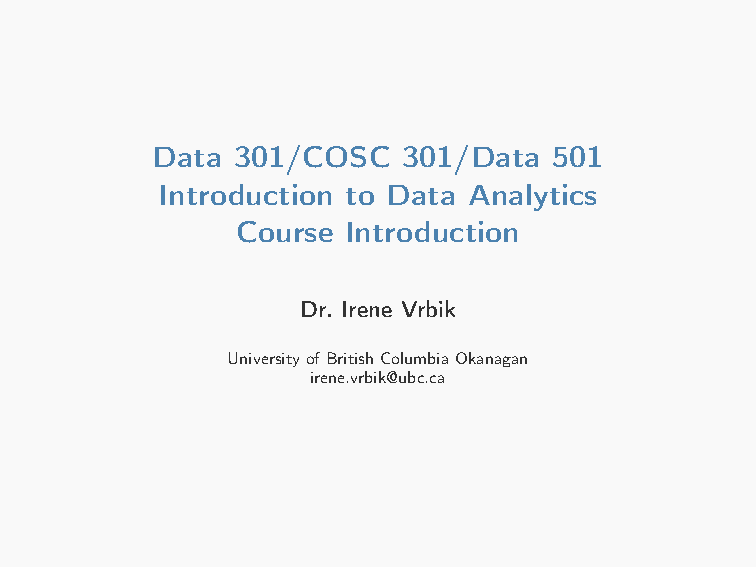
\includepdf[pages=-]{01Intro}
%\includepdf[pages=-]{02DataRepresentation.pdf}
%\includepdf[pages=-]{03ExcelPartIBeamer.pdf}
%\includepdf[pages=-]{03ExcelPartII.pdf}
%
\includepdf[pages=-]{04ExcelVBA.pdf}
%\includepdf[pages=-]{05Databases.pdf}
%\includepdf[pages=-]{05DatabasesII.pdf}
%\includepdf[pages=-]{06CommandLine.pdf}


\section{List of Topics}


\begin{table}[h]
\caption{Key}
\begin{center}
\begin{tabular}{|c|l|}
\hline
{\tt ***} & Extremely important\\
 {\tt **} & Assignment question or major topic\\
  {\tt *} &Important topic which probably should be tested\\
    -& (no stars) topic covered but probably won't be tested\\
\sout{strikethrough} &  items will (definitely) not be covered \\
\hline
\end{tabular}
\end{center}
\label{default}
\end{table}%



\subsection{Introduction (01Intro)}

\begin{itemize}
\item[*]  what is data analysis? what does a data analyst do?
\item[*] importance of data analytics
\end{itemize}



\subsection{Data Representation (02DataRepresentation)}

\begin{itemize}
%    \item[-] using the correct terminology.
\item[*]Define: computer, software, memory, data, memory size/data size, cloud
\item[*]Explain "Big Data" and describe data growth in the coming years.
\item[*] Compare and contrast: digital versus analog
  \item[-] Briefly explain how integers, doubles, and strings are encoded.
\item[*] Convert integer into unsigned binary
\item[] \sout{Convert real number into float}
\item[*] Understand why ASCII table is required for character encoding.
\item[*] Explain why Unicode is used in certain situations instead of ASCII.
\item[**] Explain the role of metadata for interpreting data.
\item[*] Define: file, file encoding, text file, binary file
   \item [-] \sout{Encode using the NATO broadcast alphabet}
      \item [-] hexidecimal
    \item[-] \sout{Discuss the time-versus-space tradeoff.}

\end{itemize}


 
\subsection{Excel (03Excel part 1 and 2)}

\begin{itemize}



\item[*] Explain what a spreadsheet is and its usefulness
 \item[**]  spreadsheet cell addressing (range notation using :)
\item[-] selecting cells in a spreadsheet
\item[-] filling, hiding
\item[*] Define and explain: formula, function, argument, concatenation
 \item[**]  Using functions, eg. concatenate, lookup, index
\item[***]  compare absolute vs. relative addresses ; use absolute addresses
\item[***] use aggregate functions
 \item[**]  use conditional formatting, format painter
 \item[**]  data and type formats
% \item[**]  Explain how spreadsheets can be used as a database.  
 \item[**]   Use sorting and filtering.
 \item[*]  Create and edit charts and use chart features: trendlines, sparklines
\item[*] Explain the usefulness of: what-if scenarios, goal seek, solver
\item[***] Use and create pivot tables and charts.
 \item[**]  Evaluate and create conditions. Use IF() to make decisions.
\end{itemize}


\subsection{Excel VBA (04 Excel VBA)}

\begin{itemize}

\item[***] Explain how to create and use macros and macro recorder
 \item[**]Explain the security issues with macros and how to handle them
 \item[-] Create and use Excel variables
\item[*] Be able to read/manipulate VBA code 
\item[] \sout{Write VBA code from scratch} %(don't need to create from scratch but you should know the general syntax)
\item[*]  Explain how a collection is different from a typical variable
\item[*]  Use/understand If/Then/Else syntax to make decisions
\item[*]  Use For loop for repetition
 \item[**] Explain how to create user-defined functions and use them in formulas
 \item[**] Difference between subroutine and functions
\item[-] Objected-oriented definitions (object, class, property, method) and objects in Excel
%\item[*]  Define: event
\item[-]List some typical user interface controls
%\item[-] Understand that Excel allows for forms and controls to be added to a worksheet which respond to events
\end{itemize}




\subsection{Relational Databases (05 Databases)}

\begin{itemize}
\item[***] Given a small database write simple queries in SQL.
 \item[**] Define: database, database system, schema, metadata
\item[***] Define: relation, attribute, tuple, domain, degree, cardinality
\item[*] SQL properties: reserved words, case-insensitive, free-format
\item[***] Be able to create a table using CREATE TABLE command %and in Microsoft Access.
\item[] \sout{GUI commands in Microsoft Access and LibreOfficeBase (i.e Design View)}
\item[**] Explain what a primary key is and what it is used for.
\item[**]  Use DROP TABLE to delete a table and its data.
 \item[**] Use INSERT/UPDATE/DELETE to add/update/delete rows of a table %and perform same actions using Microsoft Access/Libre Office Base user interface.
 \item[*] ALTER TABLE for adding columns
\item[***] Execute queries using SQL SELECT %and using Microsoft Access user interface.
  \item[**] SELECT DISTINCT for returning only unique values
 \item[**]Sort rows using ORDER BY. Use LIMIT/TOP to keep only the first (top) N rows.
 \item[**] Use GROUP BY and aggregation functions for calculating summary data.
  \item[**] HAVING for filtering after GROUP BY.
\end{itemize}

%\subsection{Command Line (06Commandline)}
%
% \begin{itemize}
% \item[**] Define command line and list some of its uses
%\item[*]  Explain the purpose of an operating system
% \item[**] Know how to open the command line window on Mac OS and Windows
% \item[**] Be able to enter commands and stop them
%\item[*]  Define: file system, folder, file
% \item[**] Explain the difference between an absolute and relative path
%\item[*]  Use command line shortcuts to save time
%\item[*]  Be able to match wildcards involving ? and *
%\item[*]  Be able to cancel a command
% \item[**] Explain standard input, standard output, and standard error
%\item[*]  Be able to use input and output redirection and pipes ($|$,$>$, $<$ , $>>$)
%\item[*]  Explain the reason for an escape symbol
%\item[*]  Define and explain the purpose of environment variables.
%\item[*]  Be able to use grep to search text files.
%\item[*]  Explain the purpose of a batch program.
% \item[-] Be able to connect to another machine using SSH. 
%\end{itemize}








\end{document}